\section{Empirical Results}
\label{sec:results}

Across all 89 tasks (267 isolated container evaluations), Supreme achieved the highest task completion (61/89, 68.5\%), the lowest aggregate wall-clock time (15.15\,h), and the lowest effective evaluation cost per successful task under recorded OpenRouter rates (\$0.489, approximately 3.4\% below Superpowers at \$0.506). Figure~\ref{fig:macro_summary} provides an executive visual comparison; Table~\ref{tab:master_scoreboard} details the complete scoreboard including infrastructure-adjusted cohorts ($N=86$, $N=85$).

\begin{table*}[t]
\centering
\caption{CARB-v4 Master Scoreboard across all 89 Terminal-Bench 2.1 tasks on Gemini 3.6 Flash High. Brackets denote Wilson 95\% score confidence intervals. Adjusted scores exclude three tasks with verified upstream container environment defects ($N=86$); a further conservative cohort excluding all four infrastructure-impaired tasks ($N=85$) is reported in Section~\ref{sec:case_studies}.}
\label{tab:master_scoreboard}
\resizebox{\textwidth}{!}{%
\begin{tabular}{lccccccc}
\toprule
\textbf{Configuration} & \textbf{Raw Solved} & \textbf{Raw Pass (\%)} & \textbf{Adjusted Pass (\%)} & \textbf{Total Time (h)} & \textbf{Avg Time / Task (s)} & \textbf{Total Tokens} & \textbf{Tokens / Solved} \\
\midrule
\textbf{Supreme} & \textbf{61 / 89} & \textbf{68.5\%} [58.3\%, 77.2\%] & \textbf{70.9\% (61/86)} [60.6\%, 79.5\%] & \textbf{15.15} & \textbf{612.9} & 34,521,410 & \textbf{565,925} \\
Superpowers by obra & 58 / 89 & 65.2\% [54.8\%, 74.3\%] & 67.4\% (58/86) [57.0\%, 76.4\%] & 18.30 & 740.2 & 34,304,008 & 591,448 \\
Baseline & 55 / 89 & 61.8\% [51.4\%, 71.2\%] & 64.0\% (55/86) [53.4\%, 73.3\%] & 16.92 & 684.3 & \textbf{31,217,863} & 567,598 \\
\bottomrule
\end{tabular}%
}
\end{table*}

\subsection{Macro Accuracy and Statistical Significance}
Supreme achieved 61 verified wins (68.5\%), compared to 58 (65.2\%) for Superpowers by obra (+3 wins) and 55 (61.8\%) for Baseline (+6 wins).

To test whether aggregate pass rate differences are statistically distinguishable, we conducted paired McNemar's tests with Edwards' continuity correction. Comparing Supreme vs.\ Superpowers yields 52 mutual passes, 22 mutual failures, 9 Supreme-only wins, and 6 Superpowers-only wins ($\chi^2 = 0.267, p = 0.605$). Comparing Supreme vs.\ Baseline yields 12 Supreme wins vs.\ 6 Baseline wins ($\chi^2 = 1.389, p = 0.239$). Comparing Superpowers vs.\ Baseline yields 12 Superpowers-only wins and 9 Baseline-only wins ($\chi^2 = 0.190, p = 0.663$).

These paired tests confirm that aggregate pass rates do not differ significantly across architectures ($p > 0.05$). The primary empirical findings emerge not from gross accuracy margins, but from operational differences in \textbf{deliberation scaling, tool ecology, and context economics}.

\begin{figure*}[t]
\centering
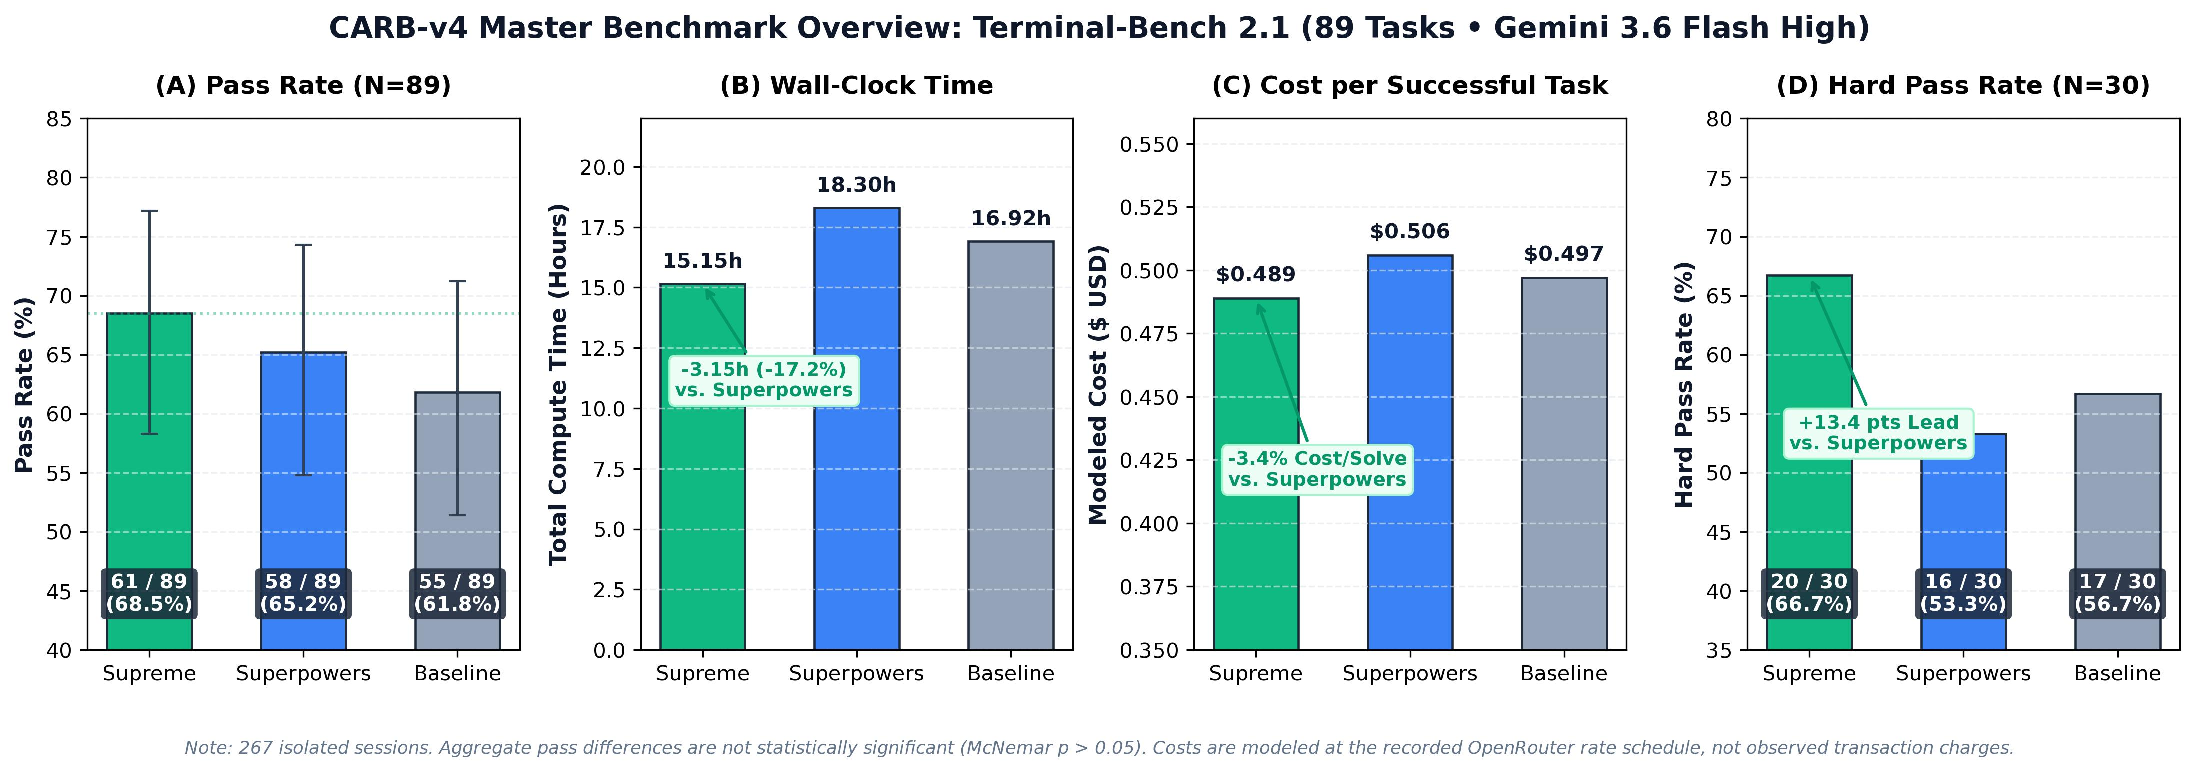
\includegraphics[width=0.98\textwidth]{figures/macro_benchmark_summary.pdf}
\caption{Benchmark outcomes and execution efficiency across all 89 Terminal-Bench 2.1 tasks (267 graded container evaluations). (A) Task completion rates with Wilson 95\% confidence intervals. (B) Total wall-clock execution time (lower is better). (C) Effective evaluation cost per successful task under recorded OpenRouter rates (lower is better). (D) Hard-task frontier pass rates ($N=30$). Supreme achieved the highest task completion (61/89, 68.5\%), the lowest aggregate wall-clock time (15.15\,h, 17.2\% lower than Superpowers), and the lowest effective evaluation cost per successful task under recorded OpenRouter rates (\$0.489, approximately 3.4\% below Superpowers). Aggregate accuracy differences are not statistically significant under paired McNemar tests ($p > 0.05$); see Section~\ref{sec:results} for full statistical analysis.}
\label{fig:macro_summary}
\end{figure*}


\subsection{Deliberation Scaling Patterns by Task Difficulty}
Across the 267 executions, the model generated 5,311,737 provider-reported deliberation tokens (\texttt{thinking\_tokens}). Table~\ref{tab:difficulty_scaling} disaggregates pass rates and mean deliberation tokens across official difficulty tiers.

\begin{table}[h]
\centering
\caption{Deliberation and Win Rates Across Complexity Strata (Wilson 95\% CIs in brackets).}
\label{tab:difficulty_scaling}
\resizebox{\columnwidth}{!}{%
\begin{tabular}{llccc}
\toprule
\textbf{Strata} & \textbf{Metric} & \textbf{Supreme} & \textbf{Superpowers} & \textbf{Baseline} \\
\midrule
\textbf{Easy} & Pass Rate & \textbf{75.0\% (3/4)} [30.1, 95.4] & 25.0\% (1/4) [4.6, 69.9] & 50.0\% (2/4) [15.0, 85.0] \\
($N=4$) & Mean Deliberation & 11,885 & 14,618 & 10,688 \\
\midrule
\textbf{Medium} & Pass Rate & 69.1\% (38/55) [56.0, 79.7] & \textbf{74.5\% (41/55)} [61.7, 84.2] & 65.5\% (36/55) [52.3, 76.6] \\
($N=55$) & Mean Deliberation & 17,035 & 17,350 & 18,090 \\
\midrule
\textbf{Hard} & Pass Rate & \textbf{66.7\% (20/30)} [48.8, 80.8] & 53.3\% (16/30) [36.1, 69.8] & 56.7\% (17/30) [39.2, 72.6] \\
($N=30$) & Mean Deliberation & \textbf{28,271} & 23,196 & 24,426 \\
\bottomrule
\end{tabular}%
}
\end{table}

Due to the small Easy strata ($N=4$), pass rates in that tier carry wide confidence intervals and are reported for completeness; no comparative inference should be drawn from them.

On Hard tasks ($N=30$), Supreme scaled mean deliberation by +66.0\% over Medium tasks (from 17.0k to 28.3k thinking tokens/task; Table~\ref{tab:difficulty_scaling}), achieving a 66.7\% pass rate (20/30). In contrast, Superpowers generated 23,196 thinking tokens/task with a 53.3\% pass rate (16/30). 

To examine this difference statistically on the Hard subset, we constructed the paired $2 \times 2$ contingency table for Supreme vs.\ Superpowers: 15 mutual passes, 9 mutual failures, 5 Supreme-only wins, and 1 Superpowers-only win. A paired McNemar test with continuity correction yields $\chi^2 = 1.500, p = 0.221$ (exact two-tailed binomial $p = 0.219$). Because this 4-task margin does not attain significance at $\alpha = 0.05$, we characterize this as a suggestive behavioral pattern (McNemar $p = 0.22$) rather than a confirmed scaling law. In Section~\ref{sec:case_studies}, we examine transcripts to investigate how dynamic documentation ingestion interacted with reasoning on these tasks.

\begin{figure*}[t]
\centering
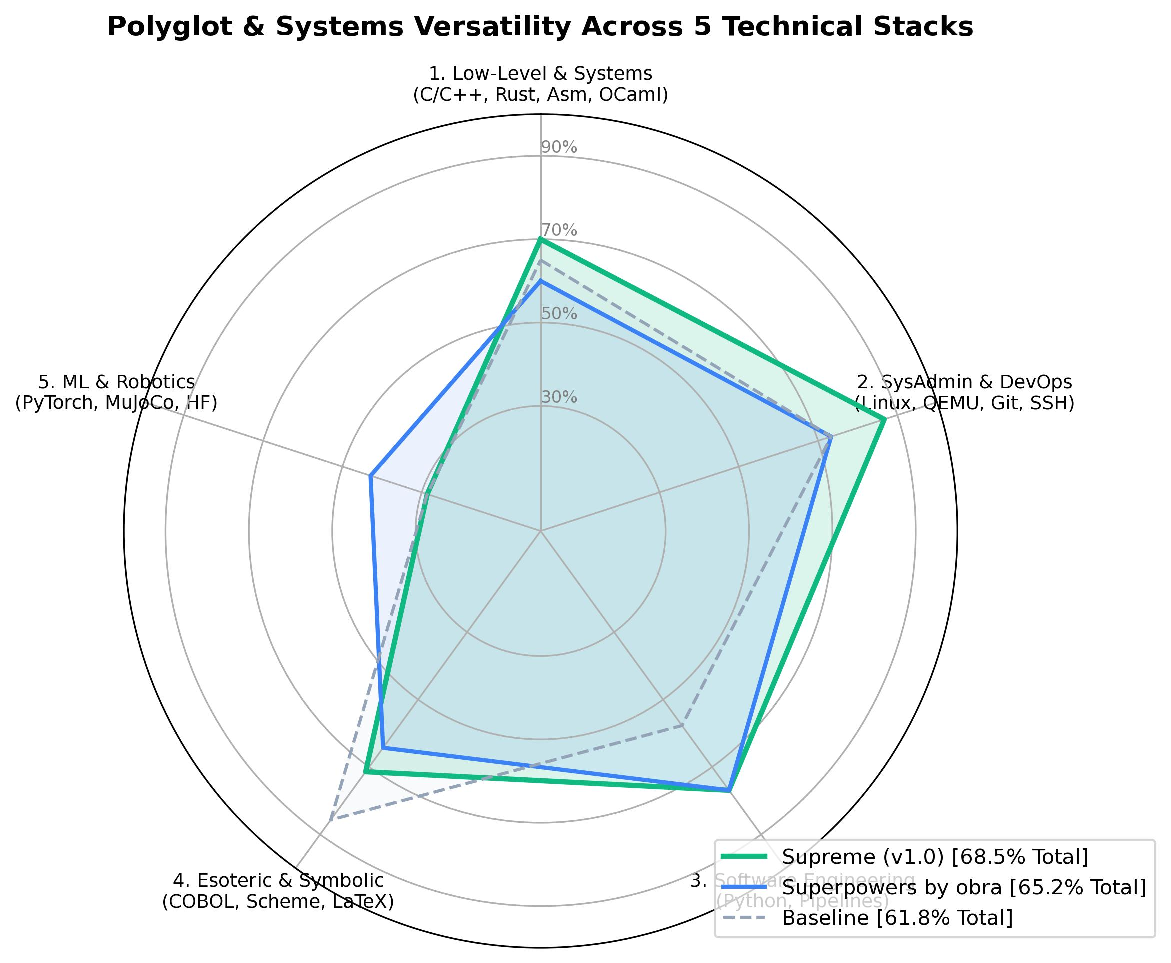
\includegraphics[width=0.48\textwidth]{figures/fig3_polyglot_5stack_radar.pdf}
\hfill
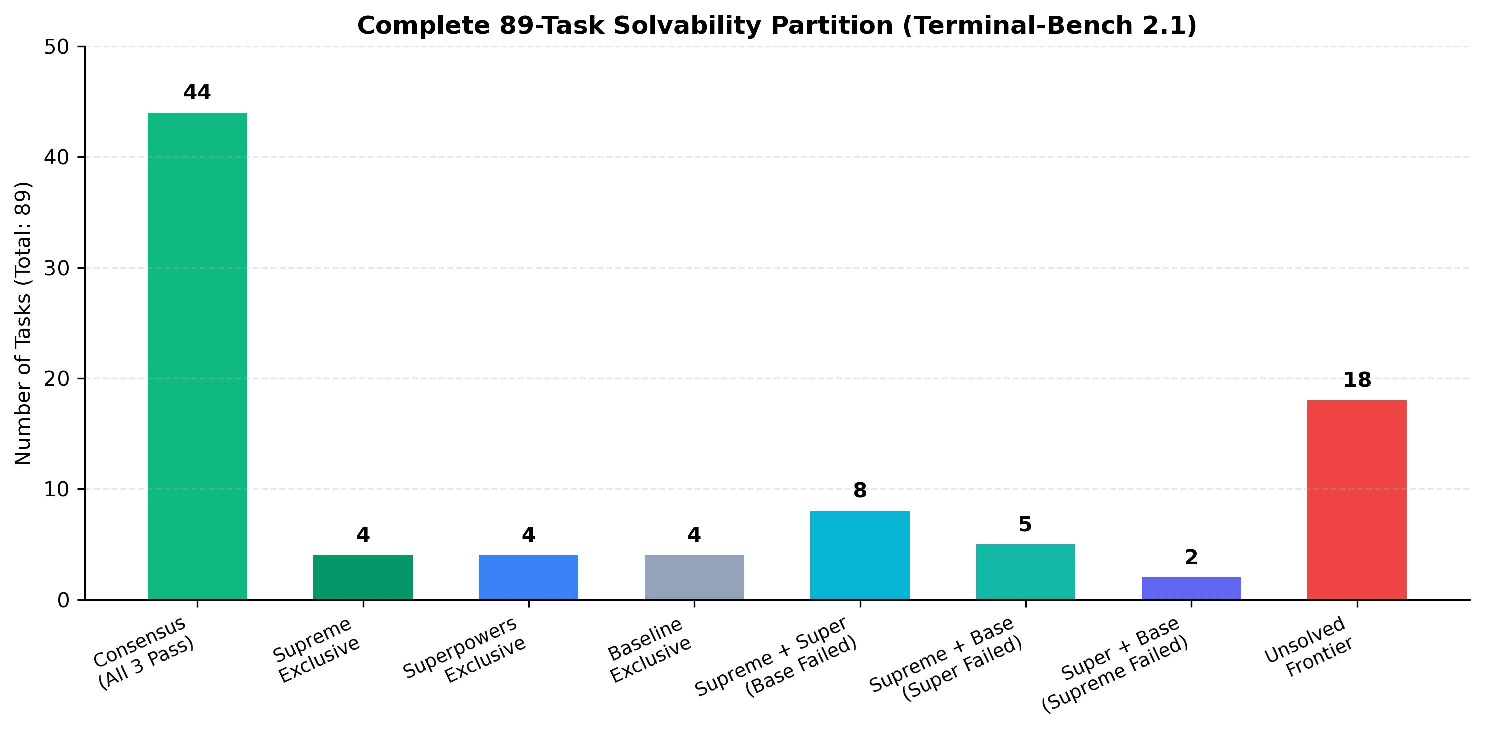
\includegraphics[width=0.48\textwidth]{figures/fig6_euler_venn_solvability_89tasks.pdf}
\caption{Domain versatility and task solvability partition. (Left) 5-Stack Polyglot performance radar. (Right) Complete 89-Task Mutual-Exclusion Partition across all eight mutually exclusive outcome subsets.}
\label{fig:polyglot_and_venn}
\end{figure*}

\subsection{Polyglot Domain Breakdown}
Table~\ref{tab:polyglot_stacks} summarizes pass rates across five engineering domains.

\begin{table}[h]
\centering
\caption{Performance Across 5 Engineering Stacks (Wilson 95\% CIs in brackets).}
\label{tab:polyglot_stacks}
\resizebox{\columnwidth}{!}{%
\begin{tabular}{lcccc}
\toprule
\textbf{Stack / Domain} & \textbf{Tasks} & \textbf{Supreme} & \textbf{Superpowers} & \textbf{Baseline} \\
\midrule
1. Low-Level Systems & 20 & \textbf{14 (70.0\%)} [48.1, 85.5] & 12 (60.0\%) [38.7, 78.1] & 13 (65.0\%) [43.3, 82.0] \\
2. SysAdmin \& DevOps & 15 & \textbf{13 (86.7\%)} [62.1, 96.3] & 11 (73.3\%) [48.1, 89.1] & 11 (73.3\%) [48.1, 89.1] \\
3. Software Engineering & 26 & \textbf{20 (76.9\%)} [57.9, 88.9] & \textbf{20 (76.9\%)} [57.9, 88.9] & 15 (57.7\%) [38.9, 74.5] \\
4. Esoteric \& Symbolic & 14 & 10 (71.4\%) [45.4, 88.3] & 9 (64.3\%) [38.8, 83.7] & \textbf{12 (85.7\%)} [60.1, 96.0] \\
5. ML \& Robotics & 14 & 4 (28.6\%) [11.7, 54.6] & \textbf{6 (42.9\%)} [21.4, 67.4] & 4 (28.6\%) [11.7, 54.6] \\
\midrule
\textbf{Total / Overall} & \textbf{89} & \textbf{61 (68.5\%)} [58.3, 77.2] & \textbf{58 (65.2\%)} [54.8, 74.3] & \textbf{55 (61.8\%)} [51.4, 71.2] \\
\bottomrule
\end{tabular}%
}
\end{table}

Due to sample sizes ($N=14$ to $26$), confidence intervals across stacks overlap substantially. Nonetheless, qualitative trends emerge:
\begin{itemize}
    \item \textbf{Low-Level Systems and SysAdmin}: Supreme demonstrated strong directional pass rates in C, Assembly, and OS administration, passing \texttt{gpt2-codegolf} (standalone C inference) and completing the 44-minute \texttt{install-windows-3.11} installation.
    \item \textbf{Esoteric \& Symbolic Tasks}: Unprompted Baseline achieved 85.7\% in Esoteric languages (Scheme, COBOL, LaTeX), outperforming both agent systems. Transcript inspection suggests that procedural guidance coincided with additional file-creation activity on these legacy toolchains, consistent with pre-trained model competency being sufficient for these task types without additional scaffolding.
\end{itemize}

\subsection{The Complete 89-Task Solvability Partition}
To examine task overlap without aggregation loss, Figure~\ref{fig:polyglot_and_venn} (Right) categorizes all 89 tasks into eight mutually exclusive subsets ($44 + 4 + 4 + 4 + 8 + 5 + 2 + 18 = 89$ tasks):
\begin{enumerate}
    \item \textbf{Consensus Passes ($N=44$)}: Solved by all three configurations.
    \item \textbf{Supreme Exclusive Wins ($N=4$)}: \texttt{fix-git}, \texttt{gpt2-codegolf}, \texttt{install-windows-3.11}, \texttt{tune-mjcf}.
    \item \textbf{Superpowers Exclusive Wins ($N=4$)}: \texttt{hf-model-inference}, \texttt{mailman}, \texttt{mteb-leaderboard}, \texttt{raman-fitting}.
    \item \textbf{Baseline Exclusive Wins ($N=4$)}: \texttt{build-pov-ray}, \texttt{gcode-to-text}, \texttt{qemu-alpine-ssh}, \texttt{regex-chess}.
    \item \textbf{Supreme + Superpowers Pass ($N=8$)}: Solved by both agent configurations but failed by Baseline (e.g., \texttt{build-cython-ext}, \texttt{cancel-async-tasks}, \texttt{fix-ocaml-gc}, \texttt{headless-terminal}, \texttt{large-scale-text-editing}, \texttt{merge-diff-arc-agi-task}, \texttt{video-processing}, \texttt{vulnerable-secret}).
    \item \textbf{Supreme + Baseline Pass ($N=5$)}: Solved by Supreme and Baseline but failed by Superpowers (\texttt{bn-fit-modify}, \texttt{circuit-fibsqrt}, \texttt{overfull-hbox}, \texttt{protein-assembly}, \texttt{rstan-to-pystan}).
    \item \textbf{Superpowers + Baseline Pass ($N=2$)}: Solved by Superpowers and Baseline but failed by Supreme (\texttt{largest-eigenval}, \texttt{model-extraction-relu-logits}).
    \item \textbf{Unsolved Frontier ($N=18$)}: Tasks unsolved by all configurations, including three tasks with verified upstream container bugs.
\end{enumerate}
One Superpowers-only pass (\texttt{mailman}) is verifier-graded (3/3 tests) with degraded agent telemetry from a stream-capture failure; it is retained as graded and flagged in the audit ledger.
This complete partition establishes that 71 of 89 tasks (79.8\%) were solved by at least one configuration, demonstrating complementary problem-solving strengths.

